\chapter{سيناريو الكشف على المنشآت}
\label{ch:01-scenario}

\section{ماذا ستنجز؟}
\label{sec:scenario-intro}

تتابع جهات الرقابة المنشآت التجارية بزيارات ميدانية تتكرر. وحين تُكتب نتيجة الزيارة على ورق أو في رسائل متفرقة، يصعب أن تعرف آخر ما تقرر بشأن منشأة، ومن راجع الكشف، وهل عُدّلت بياناتها بعد الزيارة.

يبني هذا الفصل في كيان رحلة واحدة من البداية إلى النهاية: تنظّم الهيكل والفريق، ثم تحفظ لكل منشأة سجلاً دائماً، ثم تُعدّ نموذج كشف يقرأ بياناتها، وأخيراً ترسل كل كشف إلى مدقق غير الباحث الذي أعدّه. وبذلك يبقى لكل منشأة سجل واحد، ولكل كشف تاريخه وقراره.

\begin{table}[H]
\centering
\caption{من يفعل ماذا؟}
\label{tab:scenario-roles}
\begin{tabularx}{\linewidth}{R{4.2cm} Y}
\rcHeaderRow
\thh{المسؤولية} & \thh{دورها في السيناريو}\\
مسؤول النظام & يبني الهيكل والتطبيق والنموذج والإجراء، ويجربها قبل أن يستخدمها الفريق.\\
رئيس فريق الكشف & يكلّف الباحث بالمنشأة ويحدد موعد الزيارة.\\
الباحث الميداني & يزور المنشأة، ويعبّئ الكشف ويرفق أدلته ويكتب توصيته، ثم يرسله إلى التدقيق.\\
مدقق الكشوف & يراجع الكشف ومرفقاته، ثم يعتمده أو يعيده للتصحيح أو يرفضه.\\
\end{tabularx}
\end{table}

هذه مسؤوليات في سير العمل، وليست أسماء صلاحيات جاهزة في النظام. وقد يتولى شخص واحد أكثر من مسؤولية، على ألا يدقق كشفاً أعدّه بنفسه.

يشرح هذا الفصل ما ستبنيه ولماذا. أما خطوات التنفيذ الكاملة، زرّاً بعد زر، فهي في الفصل \ref{ch:01b-build}.

\begin{rcnote}[مثال: مديرية الواحة]
تنظّم مديرية الواحة لحماية المستهلك زياراتها في تطبيق واحد. يكلّف خالد العلي، رئيس فريق الكشف، الباحثة ليلى منصور بالكشف على «فرن السنابل»، وتراجع رنا يوسف الكشف بعد إرساله. والمديرية وأشخاصها مثال افتراضي نستخدمه في الدليل كله.
\end{rcnote}

\begin{figure}[H]
\centering
\begin{tikzpicture}[node distance=0.5cm]
\node[stepBox] (a) {\RL{تنظيم الهيكل والفريق}};
\node[stepBox,below=of a] (b) {\RL{سجل دائم لكل منشأة}};
\node[stepBox,below=of b] (c) {\RL{نموذج كشف\\مرتبط بالمنشأة}};
\node[stepBox,below=of c] (d) {\RL{مسار الكشف\\من التكليف إلى القرار}};
\node[stepBox,below=of d] (e) {\RL{تجربة كل قرار\\قبل الاستخدام}};
\draw[flowsTo] (a) -- (b);
\draw[flowsTo] (b) -- (c);
\draw[flowsTo] (c) -- (d);
\draw[flowsTo] (d) -- (e);
\end{tikzpicture}
\rclegend
\caption{مراحل بناء السيناريو}
\label{fig:scenario-build-order}
\shotnote{يرتب المخطط مراحل البناء بحسب اعتماد كل منها على ما قبلها: فنموذج الكشف يحتاج إلى سجل المنشأة ليقرأ بياناتها، ومسار الكشف يحتاج إلى نموذج يُرسَل وإلى مدقق محدد يراجعه. ولا يبدأ الفريق العمل الفعلي إلا بعد تجربة الاعتماد والإعادة والرفض.}
\end{figure}

وتعني «منشأة موثّقة» في هذا الدليل أن كشفها اعتُمد داخل التطبيق وحُدّثت بياناتها بعد الاعتماد. ولا تعني إصدار سجل تجاري أو ترخيص؛ فتلك معاملة مستقلة لها شروطها.

\section{نظّم الهيكل والفريق}
\label{sec:scenario-team}

يبدأ السيناريو بمعرفة من يعمل وأين. فالوحدات التنظيمية تبيّن كيف يتوزع العمل، والمنصب يحدد مكان الوظيفة في هذا الهيكل، والتعيين يربط الشخص بالمنصب. وبذلك يعرف النظام من الباحث ومن المدقق قبل أن يصل أي كشف.

\begin{rcnote}[مثال: مديرية الواحة]
تقع «دائرة الرقابة الميدانية» تحت «مديرية الواحة لحماية المستهلك». وفيها منصب «باحث ميداني أول» تشغله ليلى منصور، ومنصب «مدقق كشوف» تشغله رنا يوسف.
\end{rcnote}

\begin{figure}[H]
\centering
\begin{tikzpicture}[node distance=0.5cm]
\node[stepBox] (a) {\RL{الوحدة التنظيمية:\\أين يقع العمل؟}};
\node[stepBox,below=of a] (b) {\RL{وصف الوظيفة:\\ما مسؤولياتها؟}};
\node[stepBox,below=of b] (c) {\RL{المنصب:\\أين مكانها في الهيكل؟}};
\node[stepBox,below=of c] (d) {\RL{العضو:\\من الشخص؟}};
\node[stepBox,below=of d] (e) {\RL{التعيين:\\من يشغل المنصب الآن؟}};
\draw[flowsTo] (a) -- (b);
\draw[flowsTo] (b) -- (c);
\draw[flowsTo] (c) -- (d);
\draw[flowsTo] (d) -- (e);
\end{tikzpicture}
\rclegend
\caption{ترتيب إعداد الهيكل والفريق}
\label{fig:scenario-team-order}
\shotnote{يجيب كل سجل في المخطط عن سؤال واحد، ويُنشأ بعد السجل الذي يعتمد عليه. فالتعيين يأتي أخيراً لأنه يربط عضواً موجوداً بمنصب موجود. أما وصف الوظيفة فاختياري للمنصب، لكنه يوضح للفريق مسؤوليات الباحث والمدقق.}
\end{figure}

\begin{table}[H]
\centering
\caption{أين تُعدّ كل سجل؟}
\label{tab:scenario-team-pages}
\begin{tabularx}{\linewidth}{R{3.6cm} Y}
\rcHeaderRow
\thh{الصفحة} & \thh{ما تسجله فيها}\\
«الوحدات التنظيمية» & الوحدة ووحدتها الأم، حتى يظهر تسلسل الجهة كاملاً، لا الأسماء وحدها.\\
«وصف الوظيفة» & عنوان الوظيفة ومسؤولياتها ومؤهلاتها، مثل مسؤوليات الباحث الميداني.\\
«المناصب» & المنصب ووحدته، ويمكن ربطه بحقل «الوصف الوظيفي».\\
«الأعضاء» & حساب الشخص وبياناته، ومنه يدخل إلى كيان.\\
«التعيينات» & ربط العضو بالمنصب، مع حالة التعيين وتاريخه.\\
«المجموعات» & جمع الأعضاء بحسب عملهم، مثل فريق الكشف ومدققي الكشوف، لتكليفهم أو منحهم صلاحيات معاً.\\
\end{tabularx}
\end{table}

\subsection{خطوات العمل والتحقق}
\begin{enumerate}
\item افتح «الموارد البشرية» ← «الوحدات التنظيمية»، وأنشئ الوحدة التي يعمل فيها الفريق مع وحدتها الأم.
\item أنشئ في «وصف الوظيفة» وصفاً للباحث الميداني وآخر للمدقق.
\item أنشئ في «المناصب» منصب الباحث ومنصب المدقق داخل الوحدة، واربط كل منصب بوصفه في «الوصف الوظيفي».
\item تأكد من وجود الباحث والمدقق في «الأعضاء»، ثم اربط كلاً منهما بمنصبه في «التعيينات».
\item أنشئ في «المجموعات» مجموعة لفريق الكشف وأخرى للمدققين.
\end{enumerate}

\textbf{تحقق:} افتح منصب الباحث، وتأكد من ظهور وحدته ومن يشغله الآن. وإذا لم يظهر الشخص، فراجع حالة التعيين وتاريخه في «التعيينات».

\section{احفظ لكل منشأة سجلاً دائماً}
\label{sec:scenario-records}

يحتاج الكشف إلى منشأة معروفة يعود إليها في كل زيارة. لذلك تبني في أدوات البناء ثلاثة أشياء مختلفة: \textbf{التطبيق} وهو المكان الذي يجمع أدوات الفريق، و\textbf{نوع السجلات} وهو شكل البيانات التي تحفظها عن كل منشأة، و\textbf{السجل} وهو منشأة واحدة ببياناتها.

\begin{rcnote}[مثال: مديرية الواحة]
تبني المديرية تطبيق «حماية المستهلك»، وفيه نوع السجلات «المنشآت التجارية». و«فرن السنابل» سجل واحد فيه، يبقى كما هو وتُضاف إليه الكشوف زيارةً بعد زيارة.
\end{rcnote}

\begin{figure}[H]
\centering
\begin{tikzpicture}[node distance=0.5cm]
\node[entity] (rec) {\RL{السجل}};
\node[entity,below=0.7cm of rec] (type) {\RL{نوع السجلات}};
\node[entity,below=0.7cm of type] (app) {\RL{التطبيق}};
\draw[dependsOn] (rec) -- (type);
\draw[dependsOn] (type) -- (app);
\end{tikzpicture}
\rclegend
\caption{التطبيق ونوع السجلات والسجل}
\label{fig:scenario-records-model}
\shotnote{يبيّن المخطط أن كل سجل ينتمي إلى نوع سجلات، وأن نوع السجلات يُعرض داخل تطبيق. لذلك تبدأ بنوع السجلات وحقوله قبل إدخال أي منشأة؛ فالحقل الذي لا يوجد في النوع لا يمكن حفظه في السجل.}
\end{figure}

\begin{figure}[H]
\centering
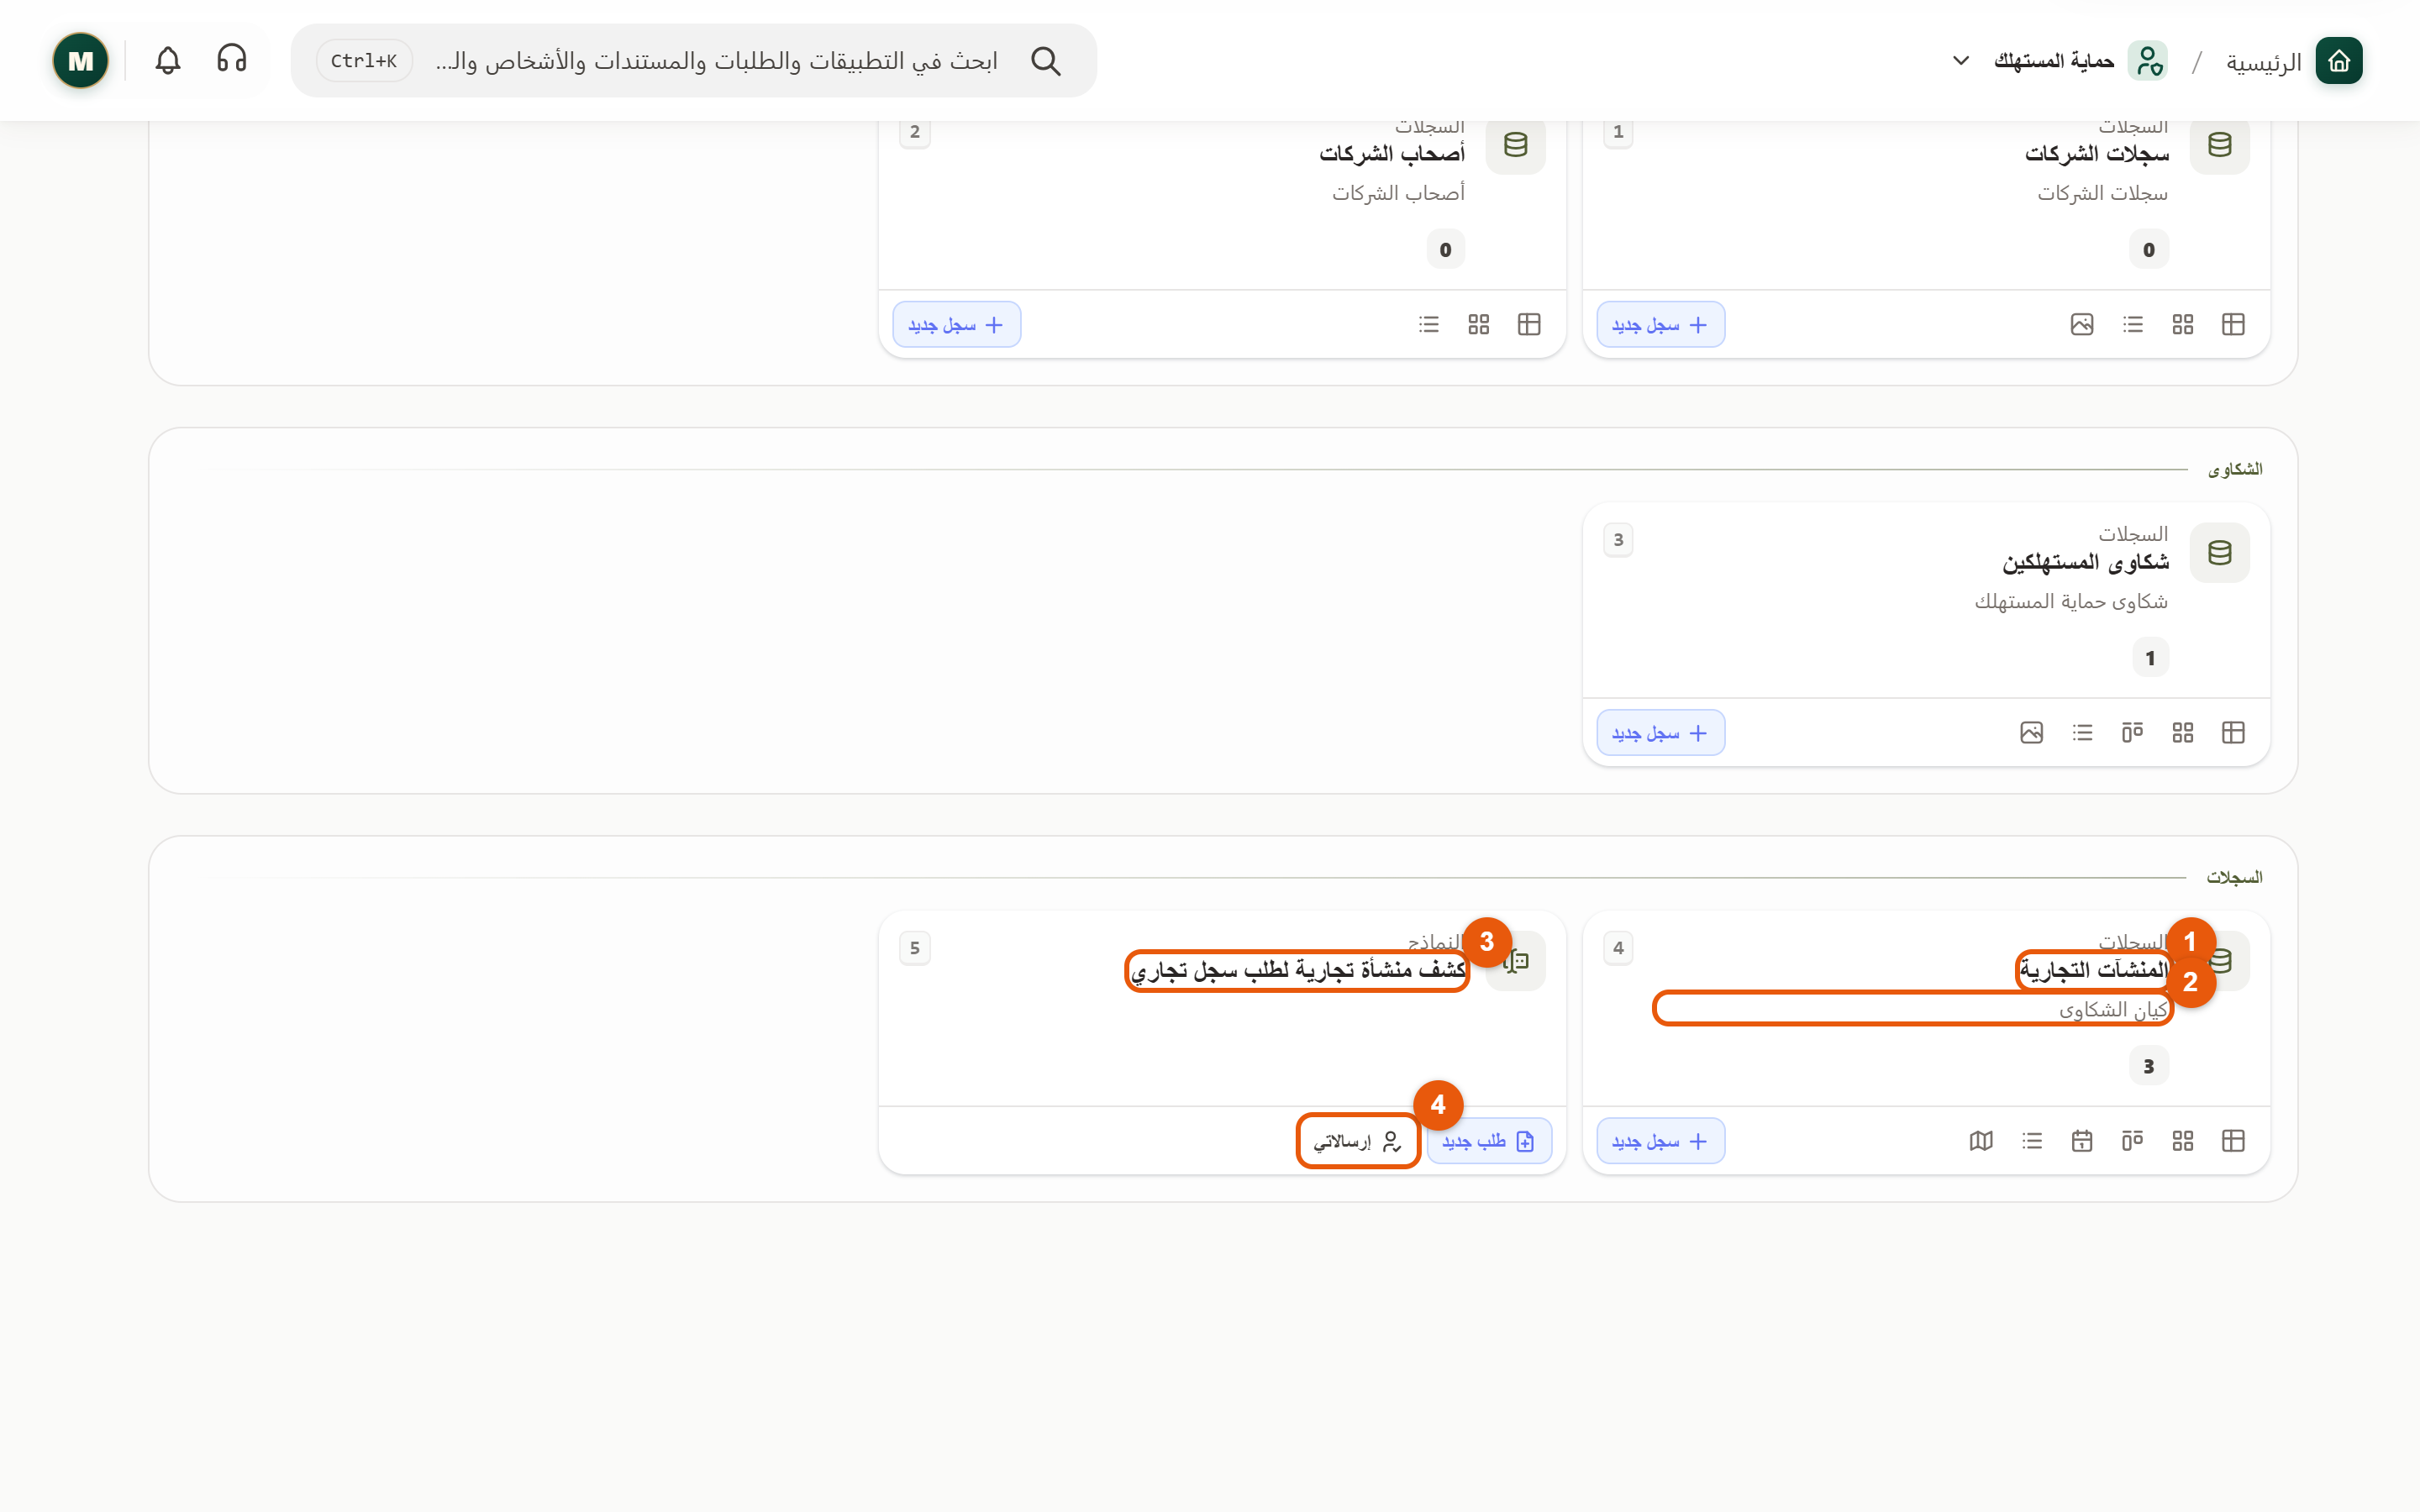
\includegraphics[width=0.95\linewidth]{assets/screens/app-home.png}
\caption{التطبيق كما يراه الفريق}
\label{fig:scenario-app-home}
\shotnote{تجمع صفحة التطبيق أنواع السجلات والنماذج في أقسام، ويمثل كل قسم جزءاً من العمل. ① اسم نوع السجلات: يفتح قائمة المنشآت. ② وصف نوع السجلات: اكتبه ليعرف الفريق محتواه. ③ نموذج الكشف داخل التطبيق. ④ «إرسالاتي»: الردود التي أرسلها المستخدم.}
\end{figure}

تسمي «ادوات البناء» أنواع السجلات «الكيانات»، وتبقى التسمية الأولى في شاشات نوع السجلات نفسها. والمقصود في الحالتين شيء واحد.

\begin{figure}[H]
\centering
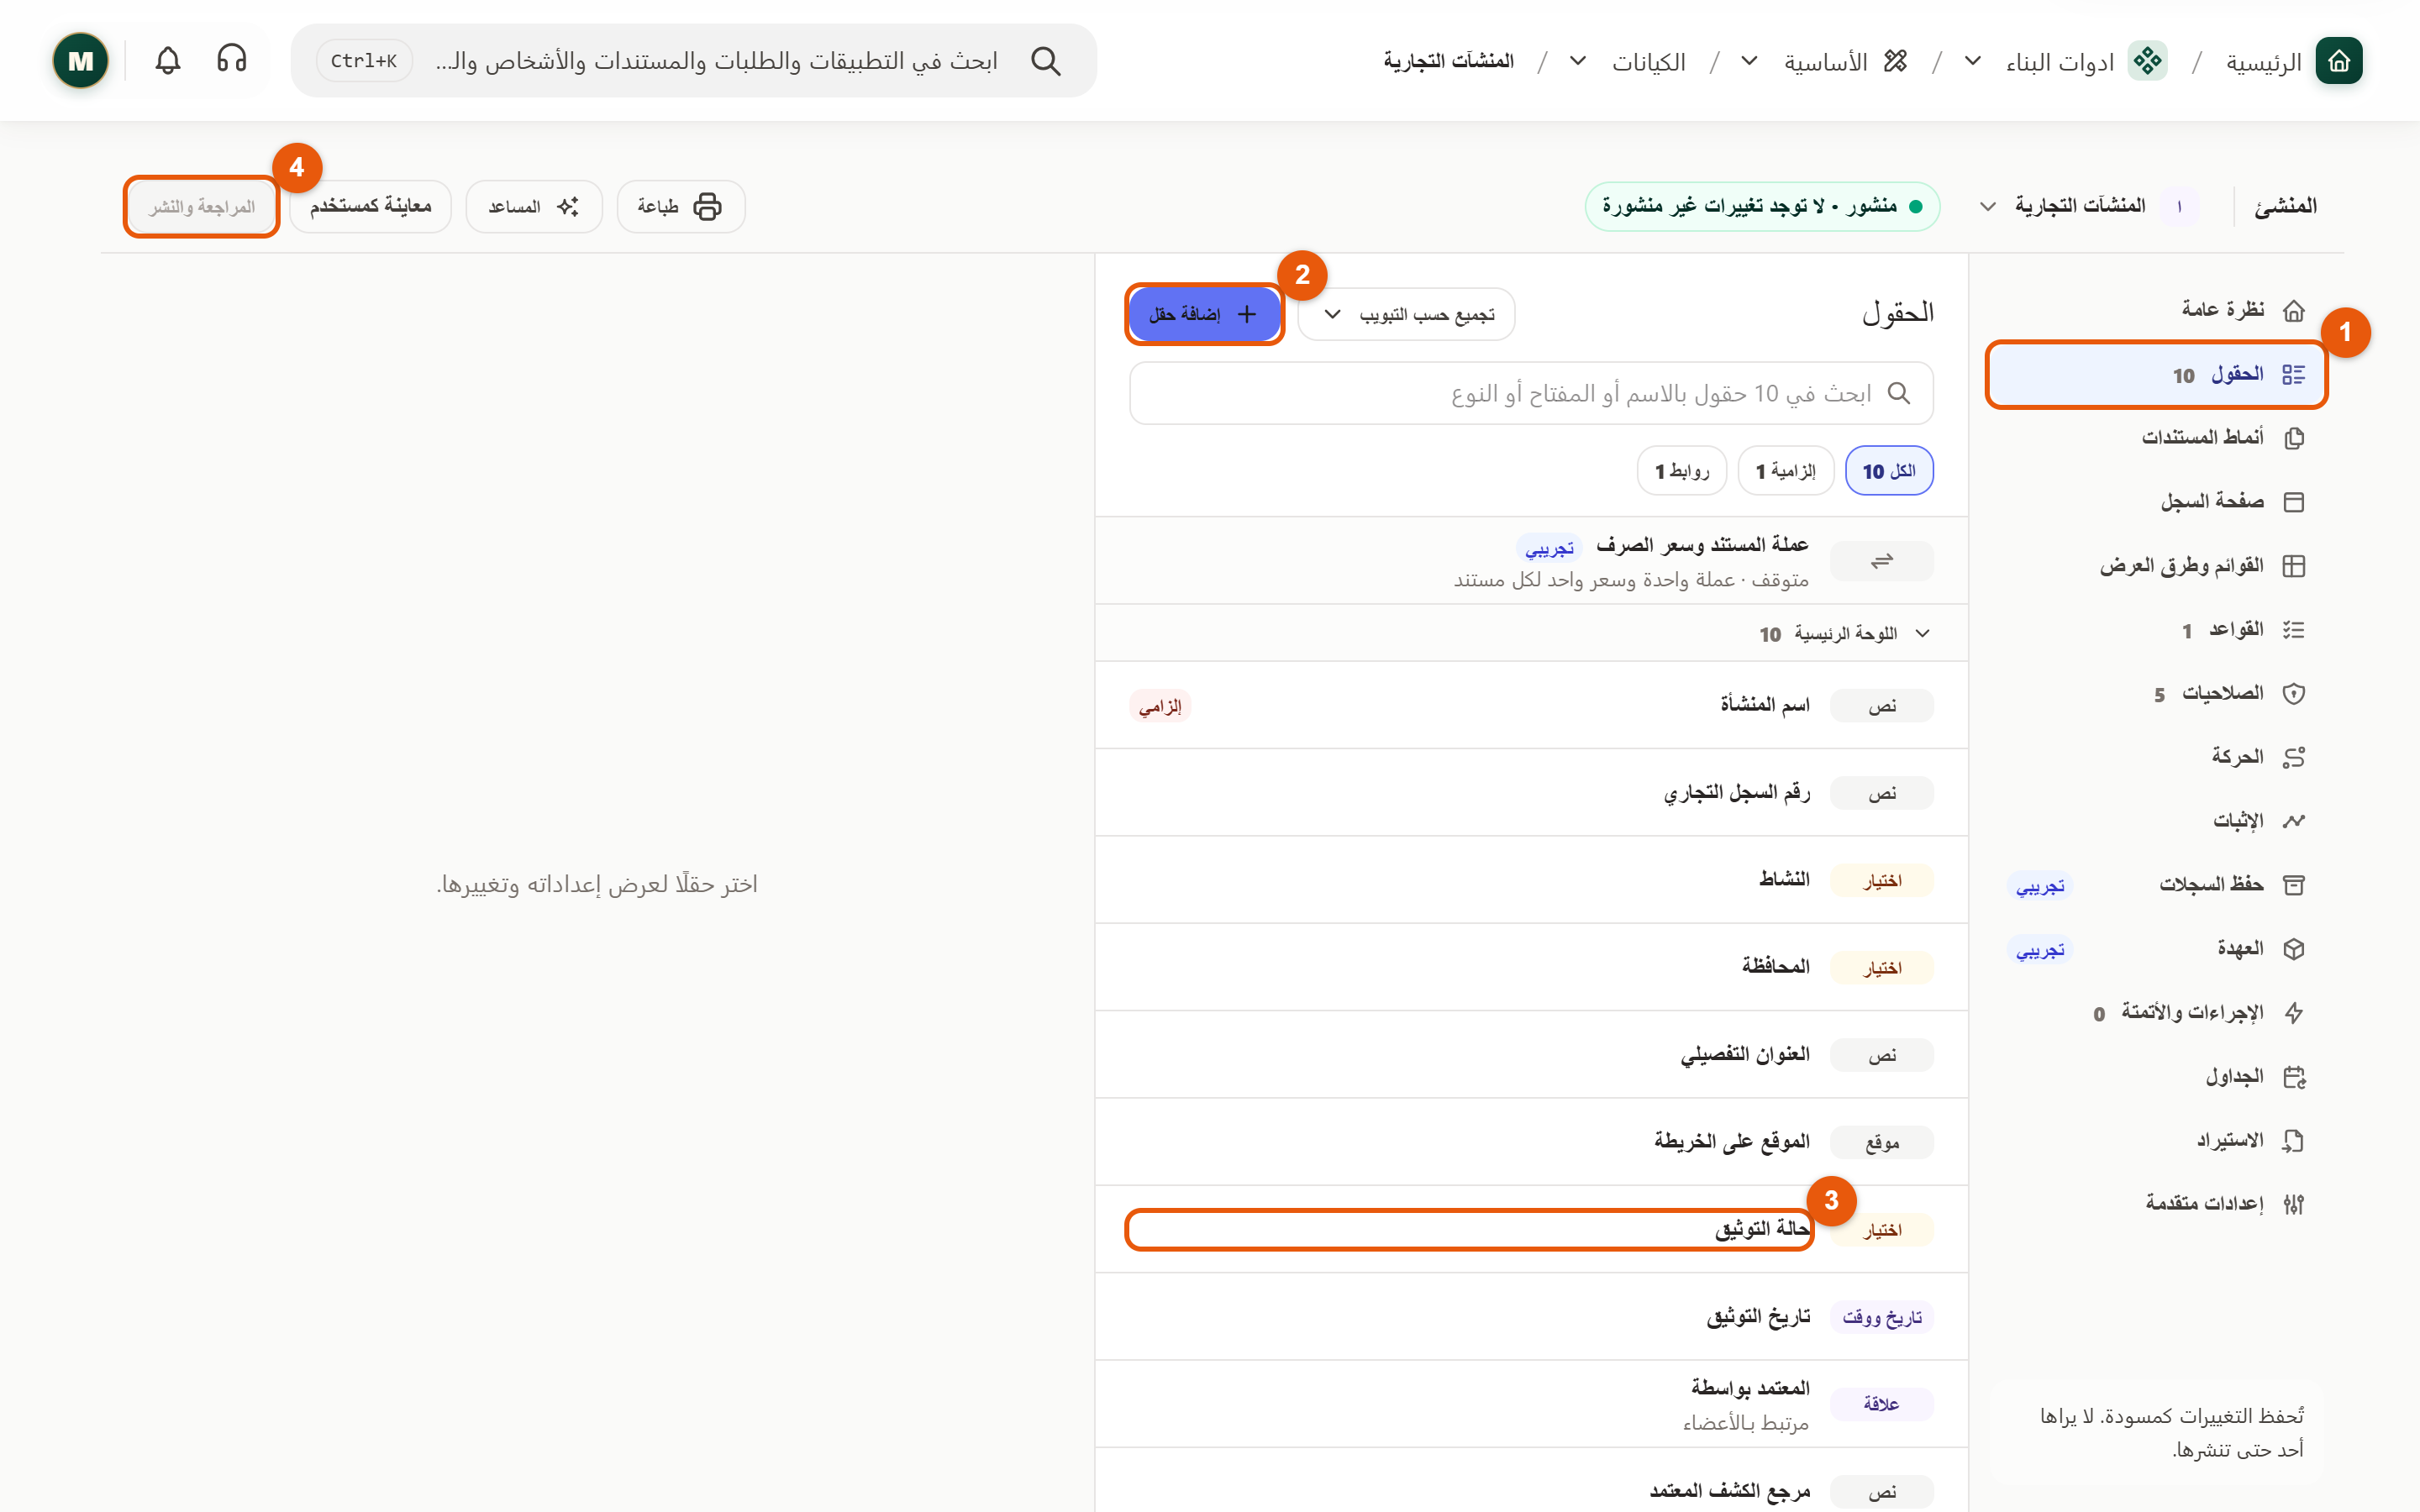
\includegraphics[width=0.95\linewidth]{assets/screens/entity-fields.png}
\caption{حقول نوع السجلات}
\label{fig:scenario-entity-fields}
\shotnote{تعرض الصفحة حقول المنشأة، ويظهر نوع كل حقل بجانب اسمه. ولا يرى أحد تعديلاتك حتى تنشرها. ① «الحقول». ② «إضافة حقل». ③ «حالة التوثيق»: حقل تكتبه نتيجة الكشف، لا الباحث. ④ «المراجعة والنشر»: يوصل التعديلات إلى الفريق.}
\end{figure}

\begin{table}[H]
\centering
\caption{حقول سجل المنشأة}
\label{tab:scenario-record-fields}
\begin{tabularx}{\linewidth}{R{3.6cm} Y}
\rcHeaderRow
\thh{المجموعة} & \thh{الحقول}\\
تعريف المنشأة & الاسم، والنشاط، ورقم السجل التجاري.\\
المكان & المحافظة، والعنوان التفصيلي، والموقع على الخريطة.\\
نتيجة التوثيق & حالة التوثيق، وتاريخ التوثيق، والمعتمِد، ومرجع الكشف الذي اعتُمد.\\
\end{tabularx}
\end{table}

لا يملأ أحد حقول «نتيجة التوثيق» يدوياً؛ إذ تُكتب بعد اعتماد الكشف كما يشرح القسم التالي. لذلك اجعلها للقراءة فقط عند الباحث من صلاحيات الحقول، حتى لا تتغير حالة المنشأة قبل القرار.

\subsection{خطوات العمل والتحقق}
\begin{enumerate}
\item افتح «ادوات البناء»، وأنشئ تطبيقاً باسم يعرفه الفريق.
\item أنشئ نوع السجلات داخل التطبيق، وأضف الحقول بحسب الجدول السابق، ثم انشره.
\item أنشئ سجلاً تجريبياً لمنشأة واحدة، وأدخل اسمها ونشاطها وعنوانها.
\end{enumerate}

\textbf{تحقق:} افتح السجل التجريبي من التطبيق، وتأكد من ظهور مجموعات حقوله الثلاث. وإذا لم يظهر حقل أضفته، فتأكد من نشر نوع السجلات بعد التعديل؛ فالتعديل غير المنشور لا يصل إلى الفريق.

\section{اربط نموذج الكشف بالمنشأة}
\label{sec:scenario-form}

نموذج الكشف هو ما يعبّئه الباحث في الزيارة: وصف واقع المنشأة، ونتائج التحقق، والمستندات والصور، وتوصيته وأسبابها. ويرتبط النموذج بالمنشأة بسؤال من نوع «سؤال سجل»، فيختار الباحث المنشأة من سجلاتها بدلاً من كتابة اسمها، ثم يقرأ النموذج بياناتها المحفوظة.

\begin{rcnote}[مثال: مديرية الواحة]
تختار ليلى «فرن السنابل» في سؤال السجل، فيظهر عنوانه المحفوظ «المزة». وتكمله في الكشف بالشارع ورقم البناء، ويبقى العنوان القديم في سجل الفرن حتى تعتمد رنا الكشف.
\end{rcnote}

\begin{figure}[H]
\centering
\begin{tikzpicture}[node distance=0.5cm]
\node[stepBox] (a) {\RL{اختيار المنشأة\\في «سؤال سجل»}};
\node[stepBox,below=of a] (b) {\RL{عرض بياناتها المحفوظة}};
\node[stepBox,below=of b] (c) {\RL{الباحث يسجّل\\ما شاهده في الزيارة}};
\node[stepBox,below=of c] (d) {\RL{الكتابة إلى السجل\\«عند الاعتماد»}};
\draw[flowsTo] (a) -- (b);
\draw[flowsTo] (b) -- (c);
\draw[flowsTo] (c) -- (d);
\end{tikzpicture}
\rclegend
\caption{كيف يقرأ الكشف من المنشأة ويكتب إليها}
\label{fig:scenario-form-link}
\shotnote{يفصل المخطط بين قراءة بيانات المنشأة وكتابتها: يقرأ النموذج البيانات عند اختيار المنشأة، لكنه لا يكتب إليها إلا بعد الاعتماد. وبذلك لا يغيّر كشف لم يُراجَع بعد بيانات منشأة يعتمد عليها الآخرون.}
\end{figure}

\begin{figure}[H]
\centering
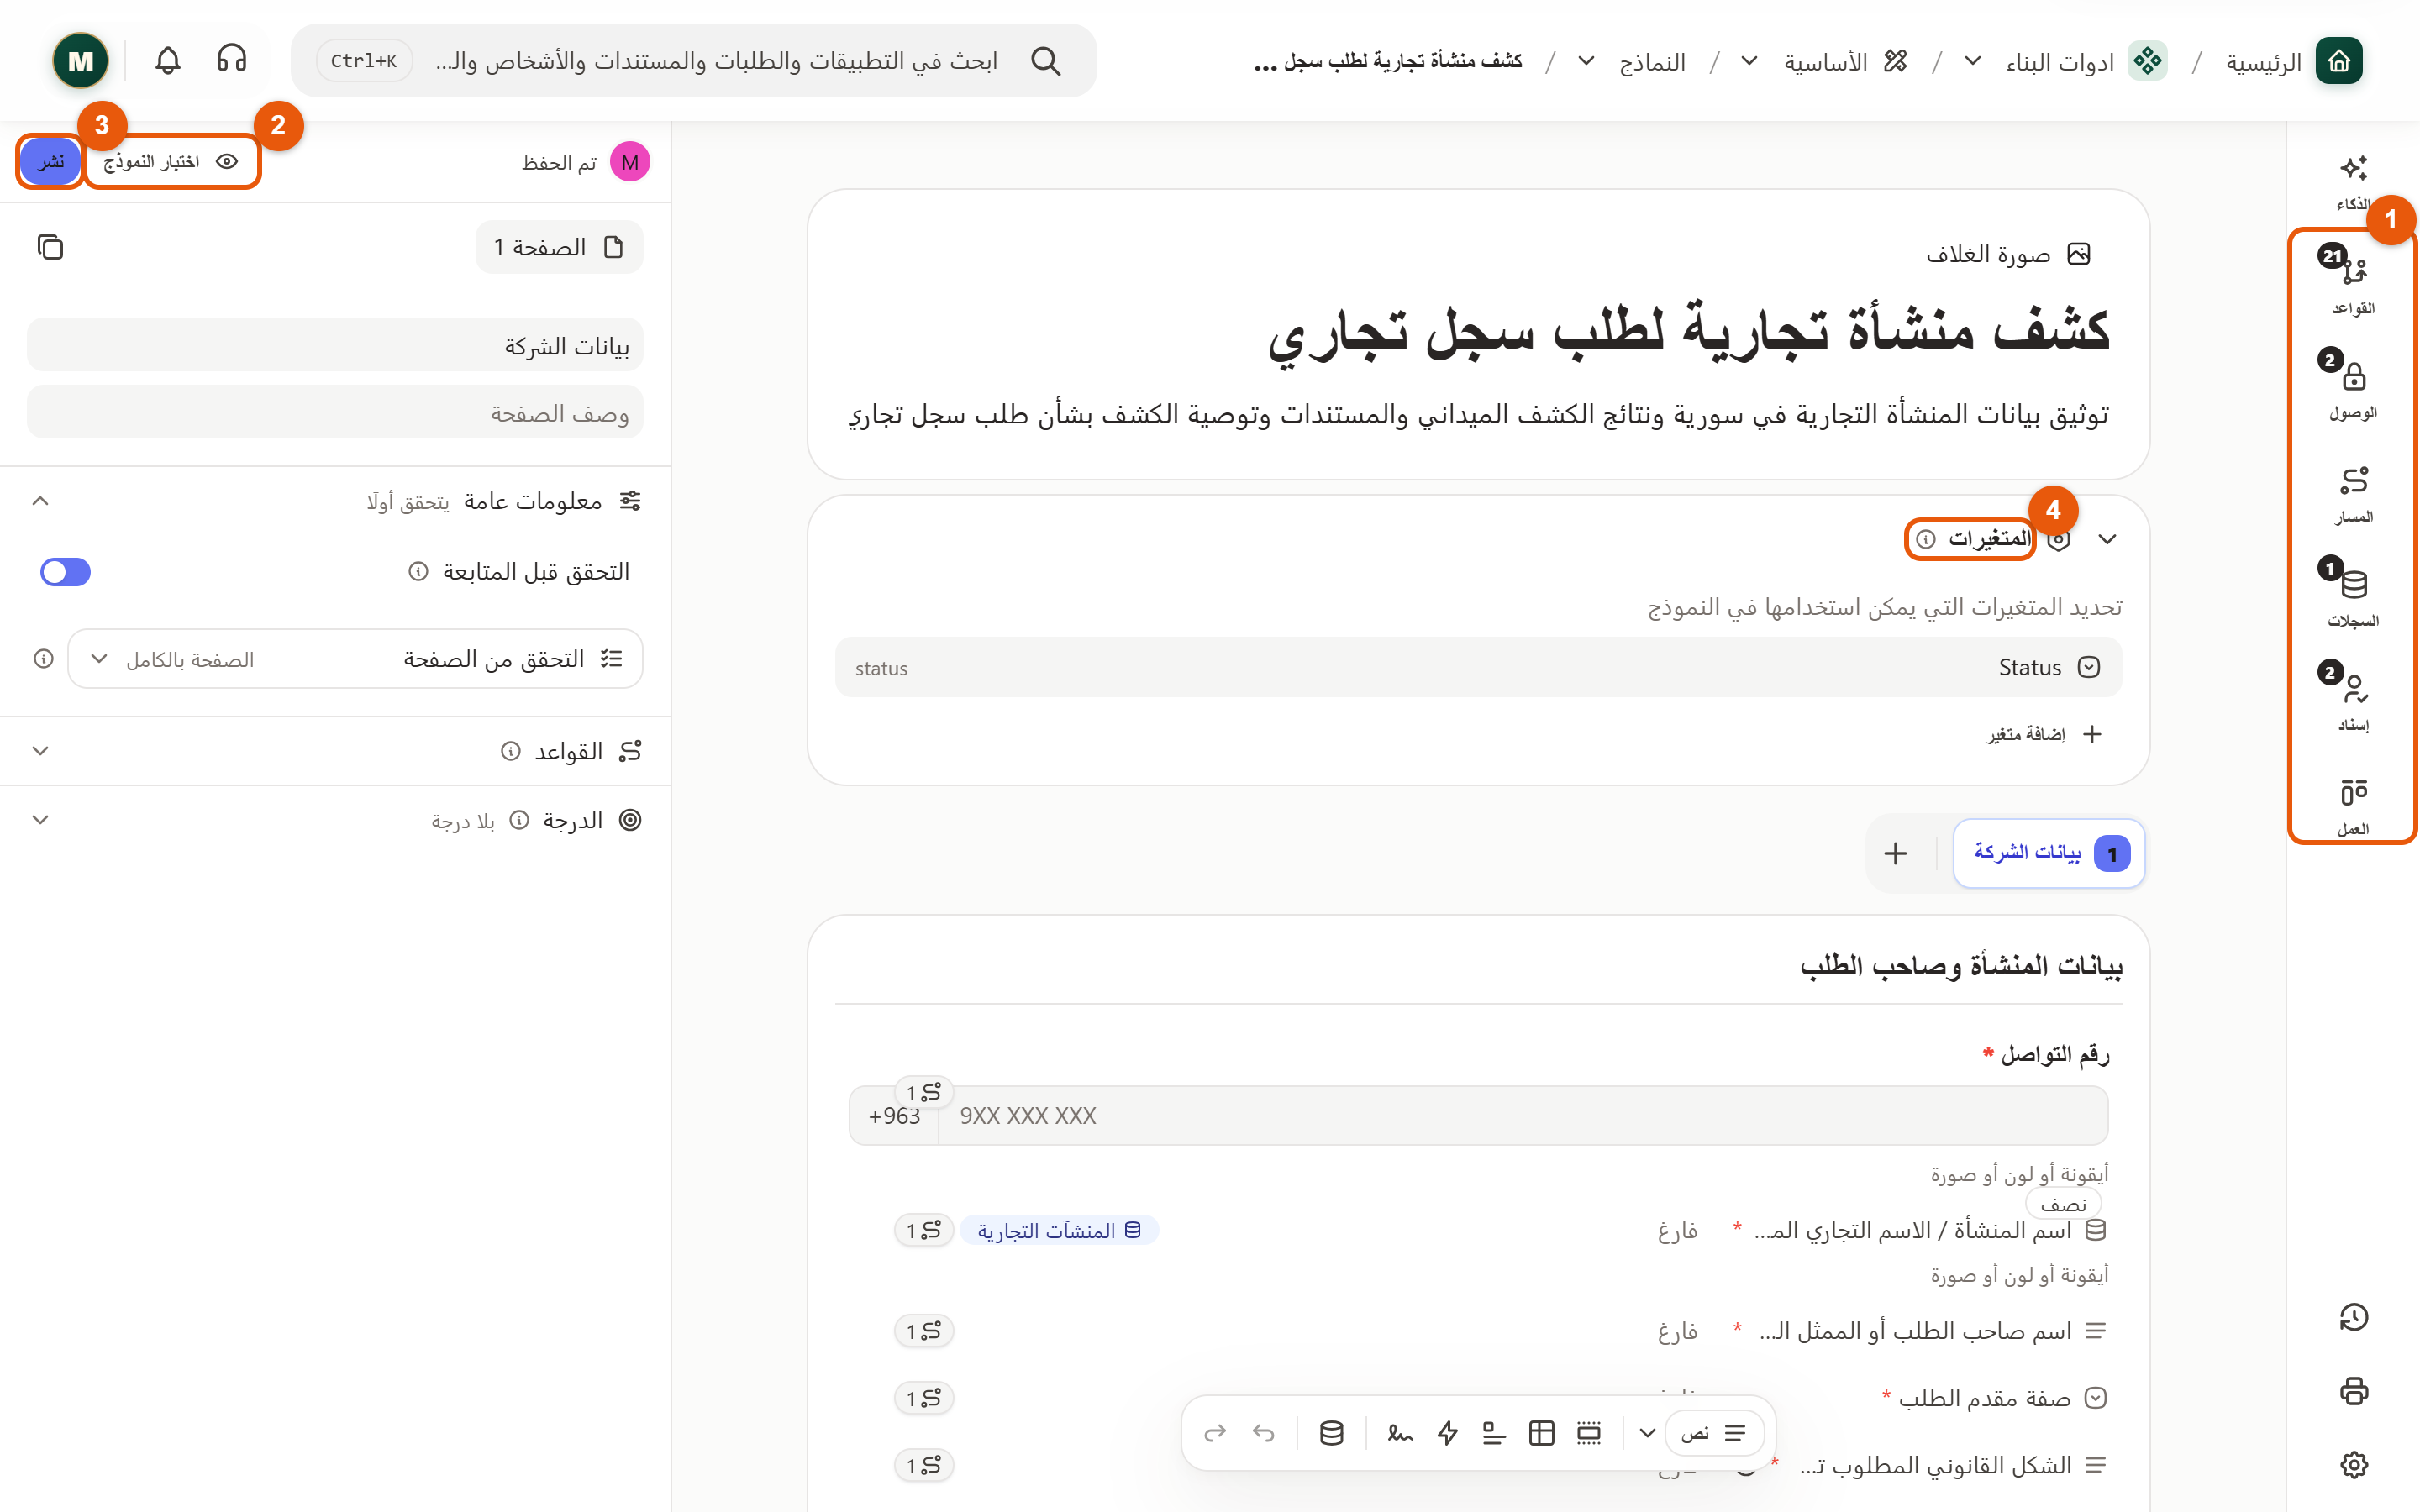
\includegraphics[width=0.95\linewidth]{assets/screens/form-builder.png}
\caption{منشئ النماذج}
\label{fig:scenario-form-builder}
\shotnote{يعرض وسط الشاشة أسئلة الكشف كما سيراها الباحث، ويفتح الشريط الجانبي إعدادات النموذج كله، وتدل الأرقام عليه على عدد ما ضُبط في كل قسم. ① «القواعد» و«الوصول» و«المسار» و«السجلات» و«إسناد» و«العمل». ② «اختبار النموذج»: جرّبه دون التأثير في الفريق. ③ «نشر»: لا يصل أي تعديل إلى الفريق قبله. ④ «المتغيرات»: قيم يستخدمها النموذج، مثل حالة الطلب.}
\end{figure}

\begin{figure}[H]
\centering
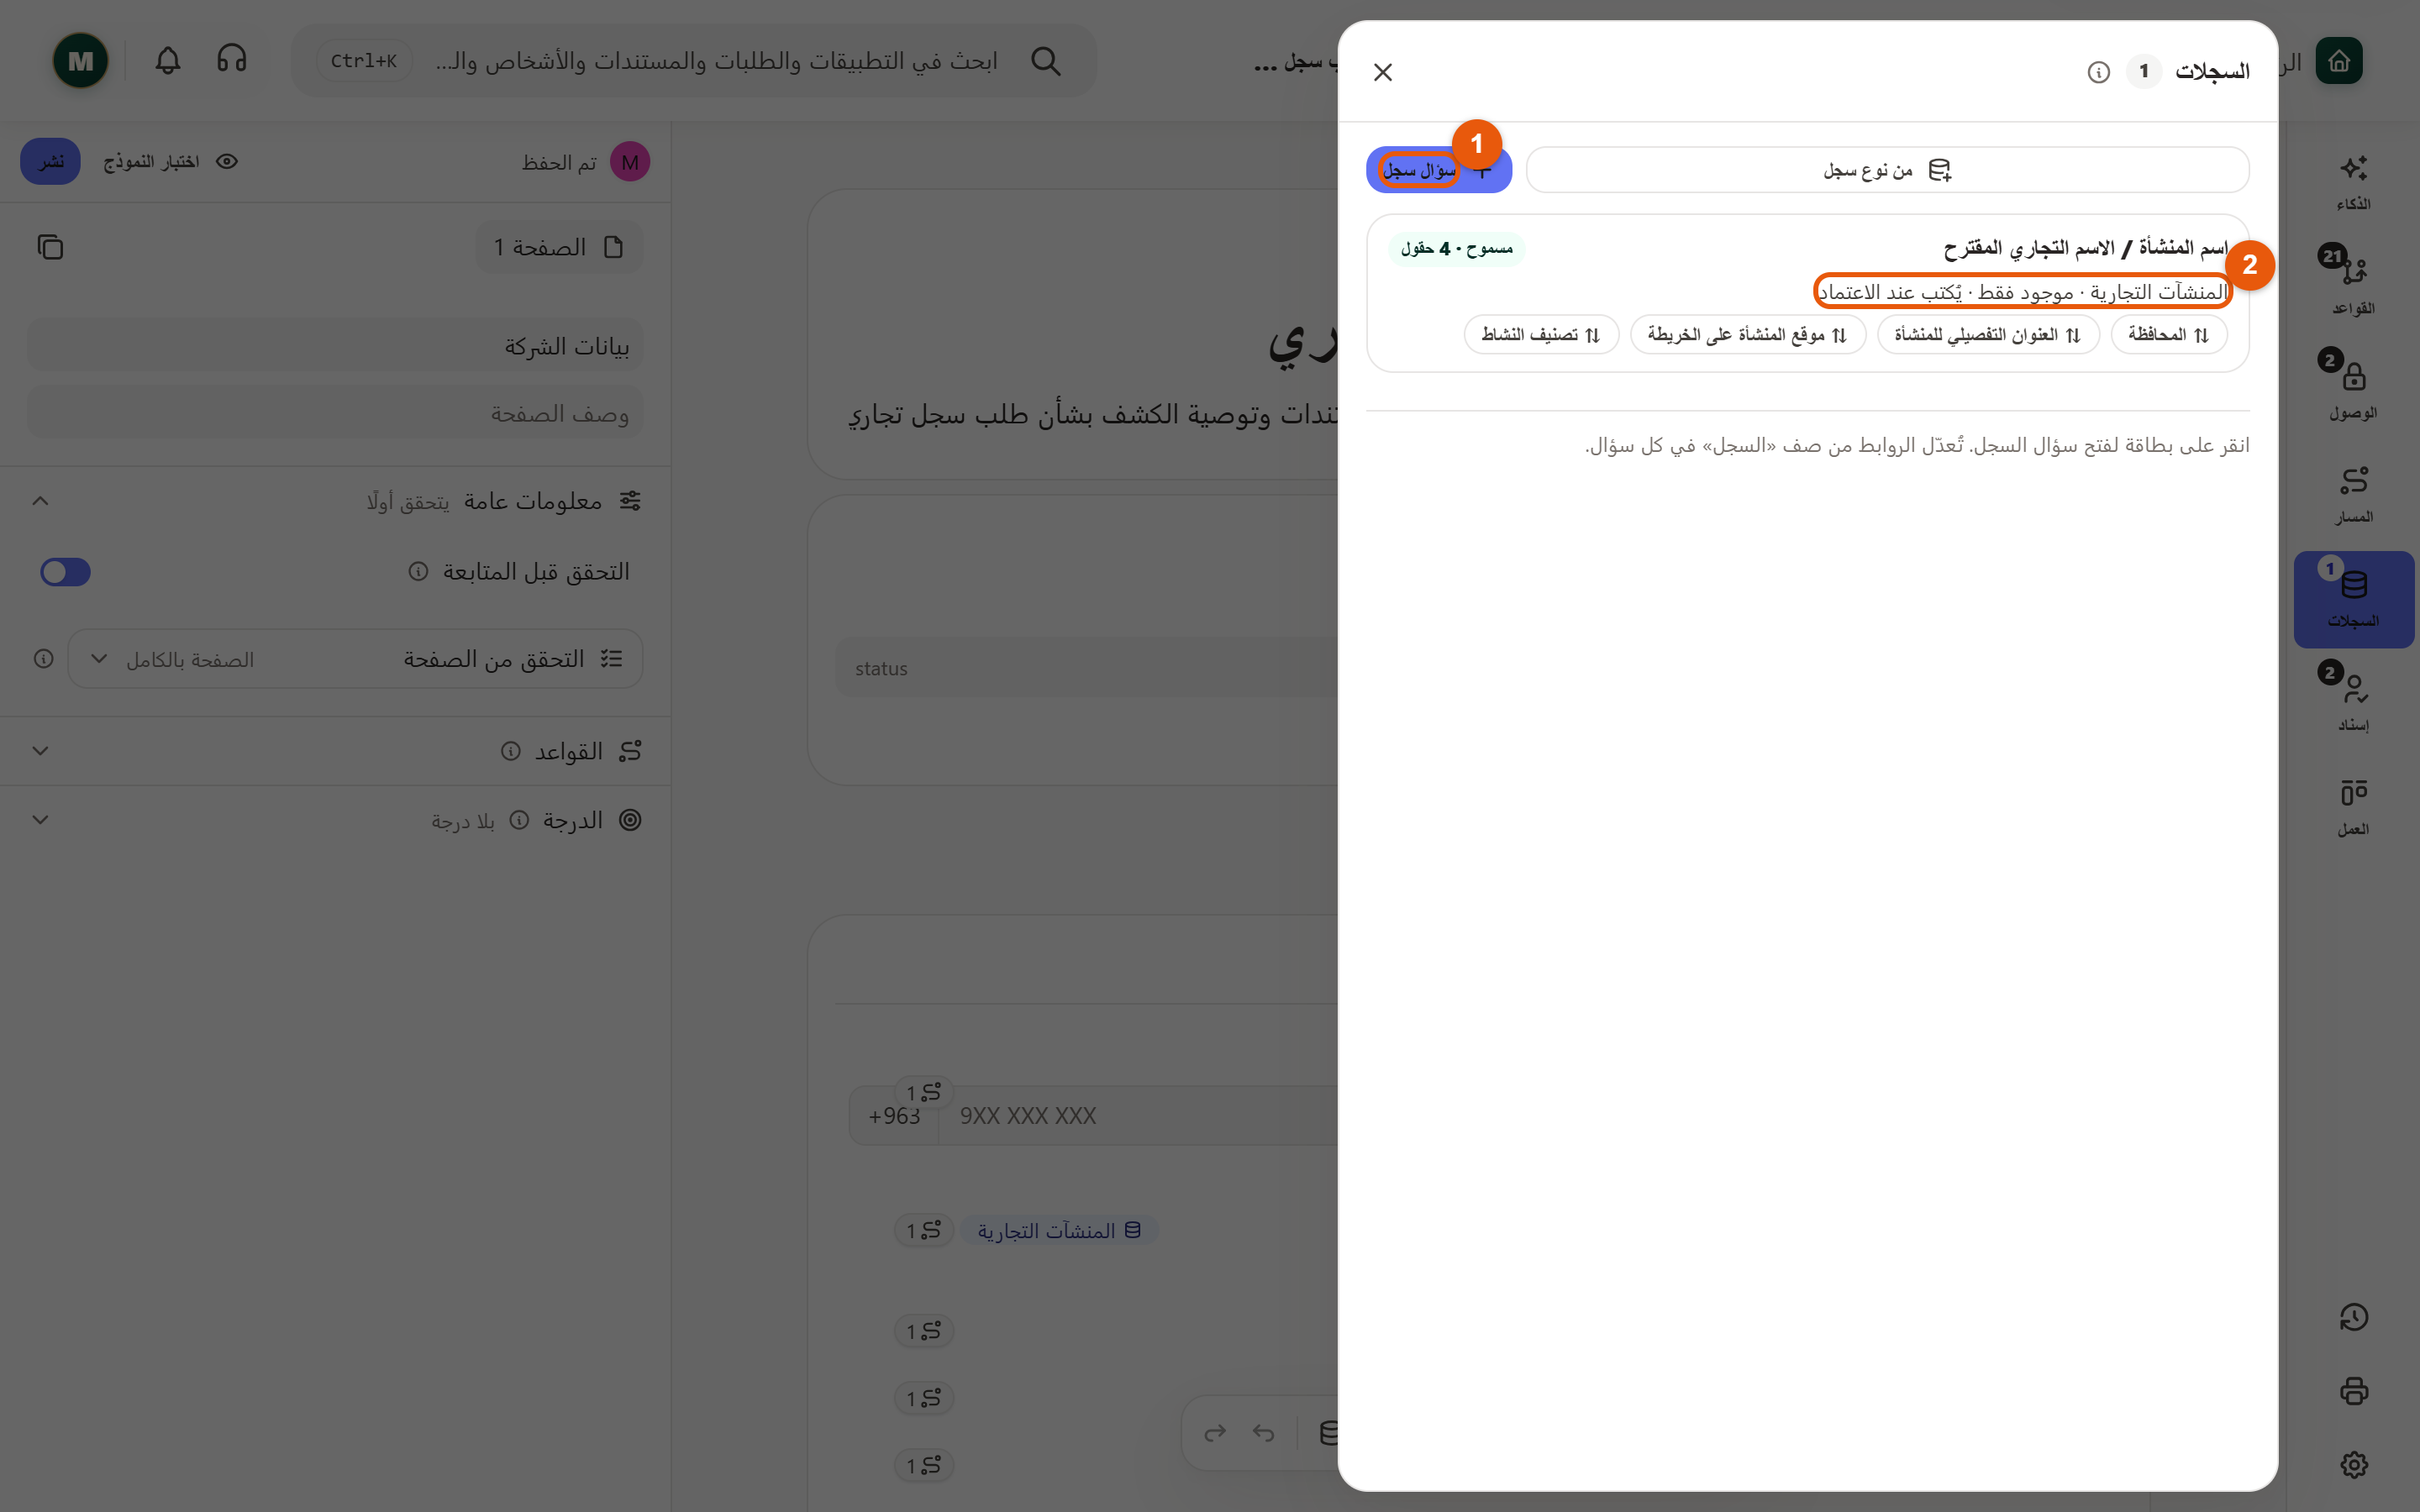
\includegraphics[width=0.85\linewidth]{assets/screens/form-records.png}
\caption{ربط النموذج بالسجل}
\label{fig:scenario-form-records}
\shotnote{تلخّص لوحة «السجلات» كل رابط في بطاقة، فتعرف ما يقرؤه النموذج وما يكتبه. ① «سؤال سجل»: يضيف سؤالاً يختار السجل. ② «يُكتب عند الاعتماد»: لا تتغير المنشأة حتى يُعتمد الكشف.}
\end{figure}

\begin{figure}[H]
\centering
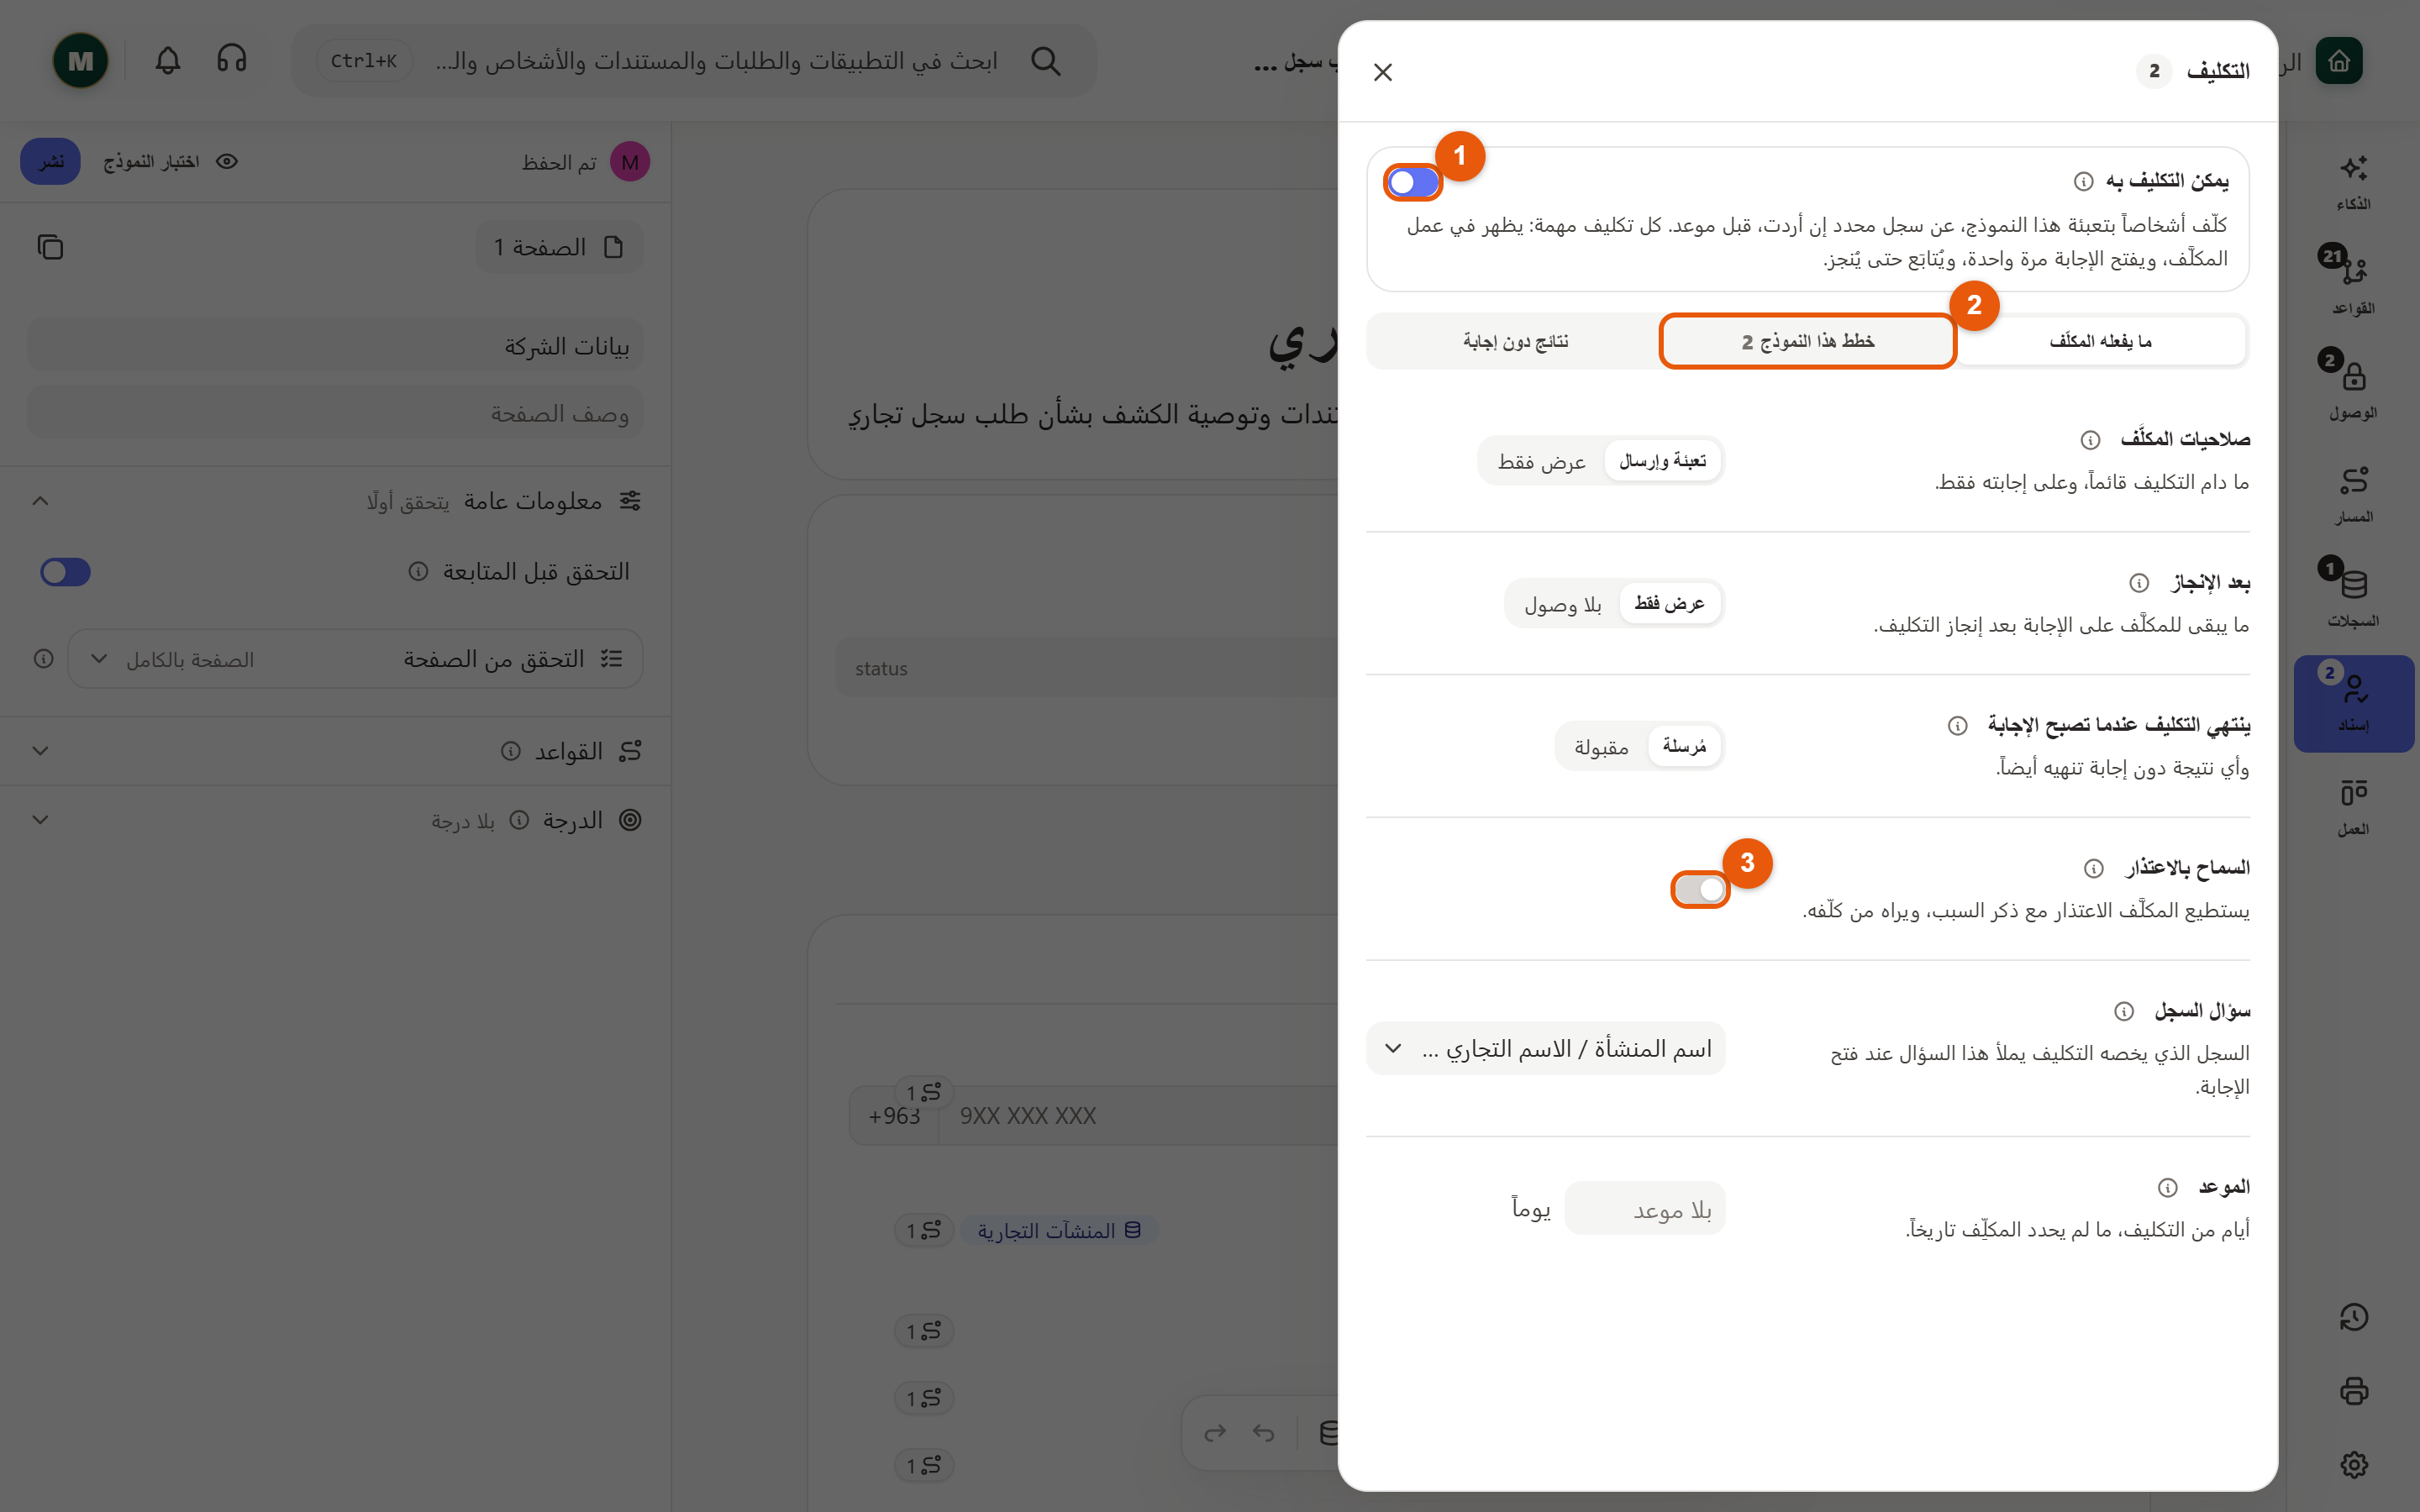
\includegraphics[width=0.85\linewidth]{assets/screens/form-assign.png}
\caption{إعدادات التكليف}
\label{fig:scenario-form-assign}
\shotnote{تحدد لوحة «إسناد» ما يحق للمكلَّف فعله ومتى ينتهي تكليفه. ① «يمكن التكليف به». ② «خطط هذا النموذج»: الخطط التي تطلقه، وإطلاقها خطوة مستقلة. ③ «السماح بالاعتذار»: يعتذر المكلَّف مع ذكر السبب، ويراه من كلّفه.}
\end{figure}

\begin{table}[H]
\centering
\caption{إعدادات النموذج التي يحتاجها الكشف}
\label{tab:scenario-form-settings}
\begin{tabularx}{\linewidth}{R{3.6cm} Y}
\rcHeaderRow
\thh{الإعداد} & \thh{لماذا تحتاجه؟}\\
«سؤال سجل» & يحدد المنشأة التي يخصها الكشف، فيُحفظ الكشف مرتبطاً بها.\\
ربط الأسئلة بحقول السجل & يعرض بيانات المنشأة على الباحث، ويحدد الحقول التي يحق للكشف تحديثها فقط.\\
الكتابة «عند الاعتماد» & تؤجل تحديث سجل المنشأة إلى ما بعد قرار المدقق.\\
«يمكن التكليف به» & يسمح بتكليف الباحث بالنموذج عن منشأة محددة وموعد محدد.\\
\end{tabularx}
\end{table}

\subsection{خطوات العمل والتحقق}
\begin{enumerate}
\item افتح النموذج في «منشئ النماذج»، ثم افتح «السجلات» وأضف «سؤال سجل» من نوع سجلات المنشآت.
\item اربط أسئلة المحافظة والعنوان والموقع بحقولها في السجل، واجعل كتابة ما يتغير منها «عند الاعتماد».
\item افتح «إسناد»، وفعّل «يمكن التكليف به».
\end{enumerate}

\textbf{تحقق:} جرّب النموذج واختر المنشأة التجريبية، وتأكد من ظهور عنوانها. ثم أرسل الكشف دون اعتماده، وافتح سجل المنشأة؛ يجب أن يبقى العنوان كما كان.

\section{سِر بالكشف من التكليف إلى القرار}
\label{sec:scenario-journey}

بعد أن صار للمنشأة سجل وللكشف نموذج، يبقى أن يمر كل كشف بالطريق نفسه: تكليف واضح، وباحث مسؤول، وقرار من مدقق مختلف عنه. وهذا الطريق المتفق عليه هو إجراء التشغيل القياسي للكشف، ويشرح الفصل \ref{ch:02-sops} كيف تكتبه وتختار أداة تنفيذه.

\begin{rcnote}[مثال: مديرية الواحة]
يكلّف خالد ليلى بكشف «فرن السنابل» يوم الأحد. تزور ليلى الفرن وتعبّئ الكشف وترسله، فيصبح «قيد التدقيق» ولا تستطيع تعديله. ثم تراجعه رنا وتقرر.
\end{rcnote}

\begin{figure}[H]
\centering
\begin{tikzpicture}[node distance=0.5cm]
\node[stepBox] (a) {\RL{رئيس الفريق يكلّف\\الباحث بالمنشأة والموعد}};
\node[stepBox,below=of a] (b) {\RL{الباحث يفتح الكشف\\عن المنشأة المحددة}};
\node[stepBox,below=of b] (c) {\RL{الباحث يعبّئ الكشف\\ويرفق الأدلة وتوصيته}};
\node[stepBox,below=of c] (d) {\RL{الإرسال إلى التدقيق:\\يتوقف تعديل الباحث}};
\node[stepBox,below=of d] (e) {\RL{المدقق يراجع ويقرر}};
\draw[flowsTo] (a) -- (b);
\draw[flowsTo] (b) -- (c);
\draw[flowsTo] (c) -- (d);
\draw[flowsTo] (d) -- (e);
\end{tikzpicture}
\rclegend
\caption{مسار الكشف الواحد}
\label{fig:scenario-journey}
\shotnote{يبيّن المخطط أن كل خطوة يؤديها شخص محدد، وأن الإرسال هو الحد الفاصل بين عمل الباحث وعمل المدقق. فبعد الإرسال لا يعدّل الباحث الكشف إلا إذا أعاده المدقق إليه للتصحيح.}
\end{figure}

\begin{table}[H]
\centering
\caption{ماذا يحدث بعد قرار المدقق؟}
\label{tab:scenario-decisions}
\begin{tabularx}{\linewidth}{R{3.6cm} Y}
\rcHeaderRow
\thh{القرار} & \thh{أثره على الكشف والمنشأة}\\
«اعتماد الكشف» & تصبح الحالة «مقبول»، وتُكتب الحقول المسموح بها إلى سجل المنشأة، ومعها نتيجة التوثيق.\\
«إعادة للتصحيح» & تصبح الحالة «بحاجة إلى تصحيح»، فيعدّل الباحث الكشف ويرسله من جديد، وتبدأ جولة تدقيق أخرى.\\
«رفض» & تصبح الحالة «مرفوض» مع سبب الرفض، وتبقى بيانات المنشأة دون تغيير.\\
\end{tabularx}
\end{table}

\textbf{تحقق:} لكل كشف صاحب واحد في كل لحظة. فإذا لم تعرف من يجب أن يتحرك الآن، فالمسار يحتاج إلى حالة أو خطوة ناقصة قبل التشغيل.

\section{جرّب كل قرار قبل الاستخدام}
\label{sec:scenario-trial}

لا يكفي أن ينجح الاعتماد مرة واحدة. جرّب السيناريو بحساب باحث وحساب مدقق، وعلى منشأة تجريبية، حتى ترى أثر كل قرار وحدود كل شخص.

\begin{rcnote}[مثال: مديرية الواحة]
تجرّب المديرية الكشف على منشأة تجريبية ثلاث مرات: تعتمده رنا مرة، وتعيده مرة، وترفضه مرة. وتحاول ليلى في كل مرة أن تعدّل الكشف بعد إرساله.
\end{rcnote}

\begin{rcchecklist}[قائمة تحقق: التجربة قبل التشغيل]
\begin{checklist}
  \item \textbf{اعتماد:} تحدّثت المنشأة الصحيحة، وظهرت فيها حالة التوثيق وتاريخه والمعتمِد.
  \item \textbf{إعادة للتصحيح:} وصلت ملاحظات المدقق إلى الباحث، وبدأت جولة تدقيق جديدة بعد إعادة الإرسال.
  \item \textbf{رفض:} حُفظ سبب الرفض، ولم تتغير بيانات المنشأة.
  \item \textbf{صلاحيات:} لم يستطع الباحث اعتماد كشفه، ولا تعديله وهو قيد التدقيق.
\end{checklist}
\end{rcchecklist}

\textbf{النتيجة:} يبقى للمنشأة سجل دائم، ولكل كشف تاريخه وقراره. وعندما تنجح البنود الأربعة، يبدأ الفريق العمل على المنشآت الفعلية.
